\footnotesize\begin{tikzpicture}
\draw[dashed](1.02,3.5)--(0,3.5)node[left]{$f_y$};
\draw[dashed](6,4.2)--(0,4.2)node[left]{$f_u$};
\draw[dashed](1,4)--(1,0)node[below]{$\varepsilon_y$};
\draw[dashed](4,3.5)--(4,0)node[below]{$\varepsilon_{sh}$};
\draw[->](-1,0)--(10,0)node[below=5mm]{strain ($\varepsilon$)};
\draw[->](0,-1)--(0,5)node[right=5mm]{stress ($f$)};
\draw[very thick,line join=round](0,0)--(1,4)node[red,thick,circle,draw,inner sep=0,minimum size=2mm]{}node[above=1mm,anchor=south west,fill=white]{upper yield stress}--(1.02,3.5);
\draw[very thick,line join=round,decoration={random steps,segment length=2.5pt,amplitude=1pt}]decorate{(1.02,3.5)--(4,3.5)node[below=4mm,midway,fill=white]{lower yield stress}};
\draw[very thick](4,3.5)to[out=30,in=180](6,4.2)node[red,thick,circle,draw,inner sep=0,minimum size=2mm]{}to[out=0,in=160](8,3.8)node[red]{\Huge\texttimes}node[right=5mm]{tension};
\node at(8,3.5){fracture};
\draw[very thick,dashed](4,3.5)to[out=40,in=185](9,5)node[right=5mm]{compression};
\draw[very thick,dashed](4,3.5)to[out=35,in=180](8,4.4)node[right=5mm]{true};
\draw[|-|](0,-.6)--++(1,0)node[midway,below=2mm,anchor=north,fill=white]{elastic range};
\draw[|-|](1,-.6)--++(3,0)node[midway,below=2mm,anchor=north,fill=white]{yield plateau};
\draw[|->](4,-.6)--++(4,0)node[midway,below=2mm,anchor=north,fill=white]{strain hardening range};
\node at(8,1.5){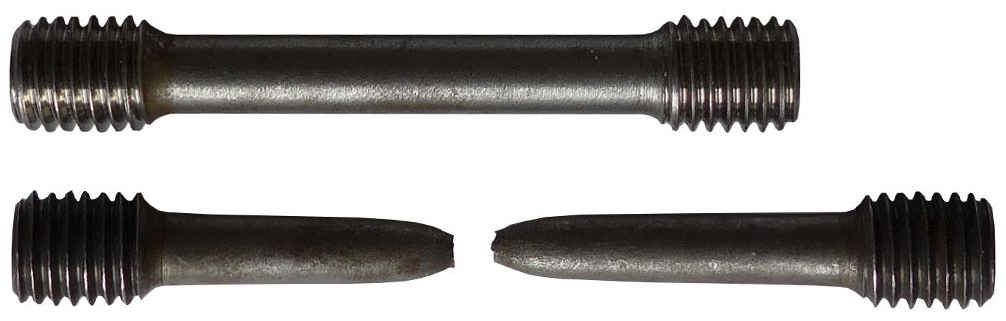
\includegraphics[width=7cm]{PIC/CH02/DT}};
\draw[line width=1mm,cc0066,->](4.2,2.1)--++(-1,0);
\draw[line width=1mm,cc0066,->](10.4,2.1)--++(1,0);
\end{tikzpicture}
